\documentclass[11pt]{beamer}
\usetheme{Luebeck}
%\usecolortheme{seahorse}
\useinnertheme{rectangles}
\useoutertheme{infolines}
\usepackage{xcolor, natbib}
\usepackage[utf8]{inputenc}
\usepackage{tikz}
\usepackage{tabularx}
\usepackage{lipsum}
\usepackage{amsmath,graphicx,dsfont}
\usepackage{graphicx}
\usetikzlibrary{shapes,backgrounds,arrows,automata,snakes,shadows,positioning, mindmap}
%===================================
\newcommand\pt{\widetilde{p}}
\newcommand{\Ccal}{\mathcal{C}}
\newcommand{\edgeunit}{1.5}
\newcommand{\emphase}[1]{\textcolor{Complement}{#1}}
\newcommand{\bleu}[1]{\textcolor{Framableulight}{#1}}
\newcommand{\pos}[1]{\textcolor{Darkgreen}{#1}}
\newcommand{\nega}[1]{\textcolor{Nicered}{#1}}
\newcommand\independent{\protect\mathpalette{\protect\independenT}{\perp}}\def\independenT#1#2{\mathrel{\rlap{$#1#2$}\mkern2mu{#1#2}}}
\newcommand{\Ncal}{\mathcal{N}}
\tikzset{%
    observed/.style={%
    scale=0.6,circle,draw=Framableulight,transform shape,fill=white,font=\Large}
}
\newcommand{\argmax}{\mathop{\mathrm{argmax}}}   
\newcommand{\backupbegin}{
   \newcounter{framenumberappendix}
   \setcounter{framenumberappendix}{\value{framenumber}}
}
\newcommand{\backupend}{
   \addtocounter{framenumberappendix}{-\value{framenumber}}
   \addtocounter{framenumber}{\value{framenumberappendix}} 
}

\makeatletter
\setbeamertemplate{footline}
{
  \leavevmode%
  \hbox{%
  \begin{beamercolorbox}[wd=.333333\paperwidth,ht=2.25ex,dp=1ex,center]{author in head/foot}%
    \usebeamerfont{author in head/foot}Raphaëlle Momal%~~\beamer@ifempty{\insertshortinstitute}{}{(\insertshortinstitute)}
  \end{beamercolorbox}%
  \begin{beamercolorbox}[wd=.333333\paperwidth,ht=2.25ex,dp=1ex,center]{title in head/foot}%
    \usebeamerfont{title in head/foot} Réseaux écologiques
  \end{beamercolorbox}%
  \begin{beamercolorbox}[wd=.333333\paperwidth,ht=2.25ex,dp=1ex,right]{date in head/foot}%
    \usebeamerfont{date in head/foot}\insertshortdate{}\hspace*{2em}
    \insertframenumber{} / \inserttotalframenumber\hspace*{2ex} 
  \end{beamercolorbox}}%
  \vskip0pt%
}
\makeatother
%===================================
\definecolor{Framableu}{RGB}{12,91,122}
\definecolor{Framableulight}{RGB}{18,144,176}
\definecolor{Nicered}{RGB}{176,18,65}
%\definecolor{Nicered}{RGB}{141,14,52}
\definecolor{Lightpink}{RGB}{229,177,218}
\definecolor{Green}{RGB}{144,176,18}
\definecolor{Lightcomplement}{RGB}{235,204,196}
\definecolor{Darkgoldenrod}{RGB}{176,144,18}
\definecolor{Darkomplement}{RGB}{122,43,12}
\definecolor{Complement}{RGB}{176,50,18}
\definecolor{Darkgreen}{RGB}{52,141,14}
%===================================
\setbeamertemplate{itemize items}[square]
\setbeamertemplate{blocks}[shadow=false]
\setbeamertemplate{caption}{\raggedright\insertcaption\par}
%===================================
\setbeamercolor{section in head/foot}{fg=white,bg=Framableu}
\setbeamercolor{subsection in head/foot}{fg=white,bg=Framableulight}
\setbeamercolor{author in head/foot}{bg=Framableu}
\setbeamercolor{item}{fg=Framableulight}
\setbeamercolor*{structure}{bg=Framableulight!20,fg=Framableulight}
\setbeamercolor*{palette secondary}{use=structure,fg=white,bg=structure.fg!75}
\setbeamercolor{section in toc}{fg=Framableu,bg=white}
\setbeamercolor{frametitle}{fg=Framableu!80,bg=white}
\setbeamercolor{block title}{fg=white, bg=Framableulight}  
%===================================
\title{Une semaine à l'observatoire PELAGIS}

\author{Raphaëlle Momal}
%\tiny{Supervision:  S. Robin$^{{1}}$ and C. Ambroise$^{\inst{2}}$  }}
%\institute[]
%{
%  \inst{1}%
 % UMR AgroParisTech / INRA MIA-Paris \\
%  \inst{2}%
%  LaMME, Evry
  %}
\date{June 23$^{\text{th}}$, 2019}

    

%#################################################################

\begin{document}

\begin{frame}
    \titlepage
    \begin{center}
    \includegraphics[width=0.2\linewidth]{logo_inra.jpg}\hspace{1cm}
	\includegraphics[width=0.2\linewidth]{agro.PNG}\hspace{0.8cm}
	\includegraphics[width=0.1\linewidth]{upsud.jpg}    
    \end{center}

\end{frame}


%====================================================================
%====================================================================
\section{Sujet}
\begin{frame}{Inférence de réseau à partir de données de comptages}

\begin{itemize}
	\item Analyse jointe de données d'abondance d'espèces (écologie, microbiologie, metagenomique )
	\item Prise en compte de covariables (caractérisant les échantillons ou l'expérience) et d'offsets (efforts d'échantillonnage..)
\end{itemize}
%\pause
\vspace{0.5cm}
\begin{block}{Réseau en écologie}
Outil pour mieux comprendre les interactions entre espèces, l'organisation des communautés.
\begin{itemize}
\item visualisation
\item gestion
\item comparaison de milieux
\item ...
\end{itemize}
\end{block}\bigskip
%\pause
\end{frame}
%====================================================================
%====================================================================


\begin{frame}{Dépendance inter-espèces}
 Reconstruction de réseau = déterminer la structure de \emphase{dépendance conditionnelle}  entre les espèces (uniquement les interactions directes).\\
 \vspace{0.5cm}
	\begin{itemize}
	\item Moins d'arêtes à analyser
	\item Éléments d'intéret plus facilement identifiables
	\end{itemize}
	\begin{columns}
\begin{column}{0.3\linewidth}\hspace{0.5cm}
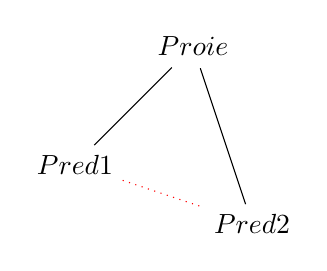
\begin{tikzpicture}	

          \tikzstyle{every edge}=[-,>=stealth',shorten >=1pt,auto,thin,draw]
		\node[] (A1) at (0*\edgeunit, 0*\edgeunit) {$Pred 1$};
		\node[] (A2) at (1.5*\edgeunit, -0.5*\edgeunit) {$Pred 2$};
		\node[] (A3) at (1*\edgeunit, 1*\edgeunit) {$Proie$};
	
		\path (A1) edge [red, dotted] (A2)
        (A1) edge [] (A3)
        (A2) edge [] (A3);
	\end{tikzpicture}\\
\end{column}
\begin{column}{0.5\linewidth}
	\begin{itemize}
	\item Le liens entre les prédateurs est indirecte : ils dépendent de la même proie.
	
\end{itemize}
\end{column}
\end{columns}
\end{frame}


\begin{frame}{Produit de la méthode}
Un réseau pondéré :\\
\vspace{1cm}
\begin{tabular}{lccc}


  \begin{tabular}{l}
		Un score par\\
		arête:
	   \end{tabular}
	   &
	   \hspace{-.05\textwidth}
	   \begin{tabular}{c}
		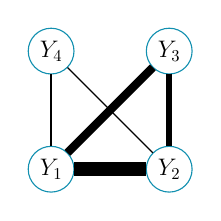
\begin{tikzpicture}
		\node[observed] (Z1) at (0*\edgeunit, 0*\edgeunit) {$Y_1$};
		\node[observed] (Z2) at (1*\edgeunit, 0*\edgeunit) {$Y_2$};
		\node[observed] (Z3) at (1*\edgeunit, 1*\edgeunit) {$Y_3$};
		\node[observed] (Z4) at (0*\edgeunit, 1*\edgeunit) {$Y_4$};
		\draw [line width=5pt] (Z1) -- (Z2); 
		\draw [line width=3pt] (Z1) -- (Z3); 
		\draw [line width=.5pt] (Z1) -- (Z4); 
		\draw [line width=2pt] (Z2) -- (Z3); 
		\draw [line width=.5pt] (Z2) -- (Z4); 
 %		\draw [line width=.5pt] (Z3) -- (Z4); 
		\end{tikzpicture}
		
	   \end{tabular}
	   &
	  \hspace{-.05\textwidth} %\pause
	   \begin{tabular}{c}
	   Seuillage \\
		$\Rightarrow$
	   \end{tabular}
	   &
	   \hspace{-.05\textwidth}
	   \begin{tabular}{c}
		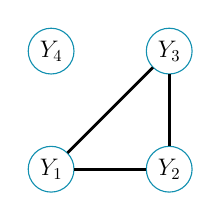
\begin{tikzpicture}
		\node[observed] (Z1) at (0*\edgeunit, 0*\edgeunit) {$Y_1$};
		\node[observed] (Z2) at (1*\edgeunit, 0*\edgeunit) {$Y_2$};
		\node[observed] (Z3) at (1*\edgeunit, 1*\edgeunit) {$Y_3$};
		\node[observed] (Z4) at (0*\edgeunit, 1*\edgeunit) {$Y_4$};
		\draw [line width=1pt] (Z1) -- (Z2); 
		\draw [line width=1pt] (Z1) -- (Z3); 
% 		\draw [line width=1pt] (Z1) -- (Z4); 
		\draw [line width=1pt] (Z2) -- (Z3); 
% 		\draw [line width=.1pt] (Z2) -- (Z4); 
% 		\draw [line width=1pt] (Z3) -- (Z4); 
		\end{tikzpicture}
	   \end{tabular}
	   \end{tabular}\\
	   \vspace{1cm}
	   Score : probabilité/fréquence de sélection 
\end{frame}
%====================================================================

\section{Application}
\subsection{Idiome du chêne}

%====================================================================
%====================================================================

\begin{frame}{Exemple : oïdiome du chêne}
\begin{columns}
\begin{column}{5cm}
\begin{figure}[htp]
\centering
\includegraphics[scale=0.07]{EA.jpg}
\caption{\textit{Pathogen Erysiphe alphitoides (EA).}}
\end{figure}
\end{column}
\begin{column}{6cm}
\begin{figure}[htp]
\centering
\includegraphics[scale=0.1]{mildew.jpg}
\caption{Feuille de chêne atteinte de l'oïdiome.}
\end{figure}
\end{column}
\end{columns}
\vspace{0.5cm}
Analyse metagénomique du microbiome des feuilles de chênes (\textit{Jakuschkin et al . 2016}).\\

\begin{itemize}
	\item 116 échantillons de 114 bactéries/champignons
	\item Efforts d'échantillonnages différents pour les bactéries/champignons
	\item Covariables : statut de l'arbre, distances au sol, au tronc et à la base de la branche
\end{itemize}
\end{frame}
%====================================================================
%====================================================================

\begin{frame}{Réseaux reconstruits}
Arêtes sélectionnées plus de 90\% du temps pour trois modèles :
    \begin{figure}[htp]
\centering
\includegraphics[width=12cm]{Oaknet_90_btw.png}
\end{figure}
Variation de densité, de dépendence du pathogène, des espèces sensibles des réseaux.
\end{frame}
%====================================================================

\subsection{REMMOA}
\begin{frame}{Recensement de Nouvelle-Calédonie}
\begin{center}

\includegraphics[width=5cm]{carte_vierge2.png} \\
\includegraphics[width=4cm]{mamif.pdf} \hspace{2cm}
\includegraphics[width=4cm]{oise.pdf}
\end{center}

\end{frame}
%====================================================================
%====================================================================

\begin{frame}{Correction d'une covariable}
\center
\includegraphics[width=12cm]{entier_covar.png}\\

\end{frame}


%====================================================================
%====================================================================

\begin{frame}{Comparaison de réseaux}
Différents niveaux d'abondance et de richesse d'espèces selon les régions :\\
\center
\includegraphics[height=4.2cm]{regionsREMMOA.png}
\includegraphics[height=4.2cm]{biodiv.png}\\
Regarder les régions séparément pour isoler les différents profils spatiaux.
\end{frame}

\begin{frame}{Comparaison de réseaux : océaniques}
\center
\includegraphics[width=12cm]{oceanique.png}\\

\end{frame}

\begin{frame}{Comparaison de réseaux : talus}
\center
\includegraphics[width=12cm]{pente.png}\\
\end{frame}


\begin{frame}{Perspectives}
Outil d'analyse exploratoire multivariée.\\

\vspace{0.8cm}

\bleu{Développements méthodologiques}
\begin{itemize}
\item Comparaison de réseaux
\item Inférence d'acteurs manquants (covariable ou espèce structurante et non observée)
\end{itemize}


\bleu{Idéologie}
\begin{itemize}
\item Développer l'interprétation des réseaux
\item Reccueillir des retours d'experts en rapport à des associations attendues
\end{itemize}

\end{frame}


\end{document}